\documentclass[a4paper,10pt]{article}
\usepackage[dvips]{color,graphicx}
\usepackage[dvips, bookmarks, colorlinks=false]{hyperref}

%opening
\title{Math650 Homework 7}
\author{Yu Huang}
\date{2006-10-12}
\begin{document}

\maketitle

\section{Question 1}
Prove that the least square estimates of $\beta$ and $\sigma^2$ are also the MLE estimates.
\begin{eqnarray}
L(\beta, \sigma^2|x) = (2\pi\sigma^2)^{-n/2}exp(-\frac{\|Y-X\| ^2}{2\sigma^2}) \nonumber \\
l(\beta, \sigma^2|x) = log(L(\beta, \sigma^2|x)) = -\frac{n}{2}log(2\pi) - \frac{n}{2}log(\sigma^2) - \frac{1}{2\sigma^2}\|Y-X\| ^2 \nonumber
\end{eqnarray}

Now let
\begin{eqnarray}
\frac{\partial{l}}{\partial{\beta}} = -\frac{1}{2\sigma^2}(-2X^T Y+2X^TX\beta)=0 \nonumber
\end{eqnarray}

This is due to
\begin{eqnarray}
\frac{\partial{\beta^TA}}{\partial{\beta}} = A \nonumber \\
\frac{\partial{\beta^TA\beta}}{\partial{\beta}} = 2A\beta \nonumber
\end{eqnarray}

We can get
\begin{eqnarray}
\hat{\beta} = (X^TX)^{-1}X^TY
\end{eqnarray}

Now put $\hat{\beta}$ into the likelihood function and let
\begin{eqnarray}
\nu = \sigma^2 \nonumber \\
\frac{\partial{l}}{\partial{\nu}} = -\frac{n}{2\nu} + 1/2\nu^{-2}\|Y-X\hat{\beta}\|^2 = 0 \nonumber
\end{eqnarray}

We can get
\begin{eqnarray} \label{eq:2}
\nu = \frac{\|Y-X\hat{\beta}\|^2}{n} = \frac{1}{n}Y^T(I-X(X^TX)^{-1}X^T)Y
\end{eqnarray}

The last equality in (\ref{eq:2}) is due to the fact that $P=X(X^TX)^{-1}X^T$ (and $I-P$) are iden-potent matrices.

\section{Question 2}
Check the example of Scottish hill races in Chapter 6 of Venables and Ripley. The influential points are one labeled in figure~\ref{f1}. Codes are appended~\ref{appendix1}

\begin{figure}
\includegraphics[angle=-90, width=1\textwidth]{figures/math650_hw7_fig1.eps}
\caption{Influential points in question 2}\label{f1}
\end{figure}

\section{Question 3}

\begin{figure}
\includegraphics[angle=-90, width=1\textwidth]{figures/math650_hw7_fig2.eps}
\caption{Influential points in question 2}\label{f2}
\end{figure}
\begin{figure}
\includegraphics[angle=-90, width=1\textwidth]{figures/math650_hw7_fig3.eps}
\caption{Influential points in question 2}\label{f3}
\end{figure}
\begin{figure}
\includegraphics[angle=-90, width=1\textwidth]{figures/math650_hw7_fig4.eps}
\caption{Influential points in question 2}\label{f4}
\end{figure}
\begin{figure}
\includegraphics[angle=-90, width=1\textwidth]{figures/math650_hw7_fig5.eps}
\caption{Influential points in question 2}\label{f5}
\end{figure}
\begin{figure}
\includegraphics[angle=-90, width=1\textwidth]{figures/math650_hw7_fig6.eps}
\caption{Influential points in question 2}\label{f6}
\end{figure}
\begin{figure}
\includegraphics[angle=-90, width=1\textwidth]{figures/math650_hw7_fig7.eps}
\caption{Influential points in question 2}\label{f7}
\end{figure}
\begin{figure}
\includegraphics[angle=-90, width=1\textwidth]{figures/math650_hw7_fig8.eps}
\caption{Influential points in question 2}\label{f8}
\end{figure}

\section{Appendix I}
\label{appendix1}
\begin{verbatim}
library(MASS)
hills.lm  = lm(time~dist+climb, data=hills)

#frame(); par(fig=c(0, 0.6, 0, 0.55))
postscript('~/script/test/math650/figures/math650_hw7_fig1.eps')
hills.fitted = fitted(hills.lm)
hills.studres = studres(hills.lm)
plot(hills.fitted, hills.studres, xlim=c(0,200), ylim=c(-2,8))
abline(h=0, lty=2)
#label the influential points
text(hills.fitted[18], hills.studres[18], row.names(hills[18,]), pos=4)
text(hills.fitted[7], hills.studres[7], row.names(hills[7,]), pos=4)
#identify(hills.fitted, hills.studres, row.names(hills))
dev.off()
\end{verbatim}

\end{document}
